% This is samplepaper.tex, a sample chapter demonstrating the
% LLNCS macro package for Springer Computer Science proceedings;
% Version 2.20 of 2017/10/04
%
\documentclass[runningheads]{llncs}
%
\usepackage{pgfgantt}

\usepackage{graphicx}
\usepackage[strings]{underscore}
\usepackage[hyphens]{url}
\usepackage{ragged2e}
\usepackage{tabularx}

\setlength{\parindent}{0in}
% Used for displaying a sample figure. If possible, figure files should
% be included in EPS format.
%
% If you use the hyperref package, please uncomment the following line
% to display URLs in blue roman font according to Springer's eBook style:
% \renewcommand\UrlFont{\color{blue}\rmfamily}
\renewcommand\refname{Literaturangaben}

\begin{document}
%
\title{Hauptprojekt \\~\\ Konzeption und prototypische Implementierung einer verteilten Autoscaling-Architektur für Cloud-Bursting mit Container-as-a-Service}
%
\titlerunning{Hauptprojekt}
% If the paper title is too long for the running head, you can set
% an abbreviated paper title here
%
\author{Christian F. Bargmann}
%
% \authorrunning{F. Author et al.}
% First names are abbreviated in the running head.
% If there are more than two authors, 'et al.' is used.
%
\institute{Hamburg University of Applied Sciences, Berliner Tor 5, 20099 Hamburg, Germany \\
	\email{christian.bargmann@haw-hamburg.de} \\
	\url{https://www.haw-hamburg.de}}
%
\maketitle              % typeset the header of the contribution
%
\begin{abstract} Cloud-Bursting ist ein Betriebsmodell, bei dem eine Anwendung in einer privaten Cloudumgebung oder einem Rechenzentrum betrieben wird, jedoch automatisch Ressourcen einer öffentlichen Cloud provisioniert werden, wenn die Nachfrage nach Rechenkapazität ansteigt. Die Entscheidung, anhand welcher Kriterien Ressourcen in eine öffentliche Cloud ausgelagert werden, wie sich die provisonierten Ressourcen in die lokal betriebene Infrastruktur integrieren lassen und welches Servicemodell des Cloud-Providers verwendet werden soll, ist in den vergangenen Jahren in den Fokus aktueller Forschung gerückt. Dieses Hauptprojekt konzeptioniert, implementiert und evaluiert eine verteilte Autoscaling-Architektur für Cloud-Bursting in Hybrid-Clouds, die automatisiert Ress\-ourcen auf Basis von Metriken als Container-as-a-Service bei mehreren Cloud-Service-Providern provisionieren und skalieren kann.
		
	\keywords{Cloud Bursting \and Cloud Computing \and Autoscaling \and \newline Container \and Software Architektur}
\end{abstract}
%
%
%
	
\section{Einleitung} \label{motivation}
	
Cloud-Bursting ist ein Betriebsmodell, bei dem eine Anwendung in einer privaten Cloudumgebung oder einem Rechenzentrum betrieben wird, jedoch automatisch Ressourcen einer öffentlichen Cloud provisioniert werden, wenn die Nachfrage nach Rechenkapazität ansteigt. Bei diesem hybriden Betriebsmodell wird die eigene Infrastruktur vollständig genutzt, so dass eine Anzahl von Servern in eigener Verantwortung und Kontrolle betrieben werden kann. Gleichzeitig besteht bei Lastspitzen die Möglichkeit, die Anwendung ganz oder teilweise in eine externe, öffentliche Cloud zu verlagern. \\
	
Die wichtigste Technologie bei Cloud-Computing zum Hosten und Verwalten von Anwendungen ist die Virtualisierung. Traditionell wird Hardware-Level-Virtualisierung, auch bekannt als Hypervisor-basierte Virtualisierung, zur Verwaltung von virtuellen Maschinen (VMs) in Cloud-Rechenzentren verwendet. Ein grosser Fortschritt in der Virtualisierungstechnologie ist die Containerisierung von Anwendungen, die auch als Virtualisierung auf Betriebssystemebene bekannt ist. Aufgrund der besseren Portabilität, des geringen Ressourcenbedarfs und der einfachen Skalierbarkeit im Vergleich zur VM-basierten Virtualisierung, hat Containerisierung in den letzten Jahren deutlich Popularitaet gewonnen. Containerisierung eignet sich für die Verwaltung von Microservices, da sie das schnelle Starten und Beenden von Containern und somit schnelle Skalierbarkeit unterstützt, während die VM-basierte Virtualisierung vergleichsweise mehr Zeit für das Starten und Beenden der VM benötigt \cite{al-dhuraibi_elasticity_2018}, \cite{abdullah_containers_2019}. Viele Cloud-Service-Provider (CSPs) bieten Container-as-a-Service Angebote an, mit denen sich Container in einer Cloud-Umgebung betreiben lassen, ohne darunterliegende Infrastruktur selbst verwalten zu muessen. \\

Trotz dieser modernen As-a-Service Angebote, ist die Umsetzung eines Hybrid-Cloud Ansatzes fuer viele Unternehmen nach wie vor eine grosse Herausforderung. Die Integration zwischen eigener Infrastruktur und den Schnittstellen der CSPs, sowie die Wahl von geeigneten Skalierungsmethoden, ohne dabei zu stark an eine bestimmte Cloud-Plattform gekoppelt zu sein, ist nicht trivial.  \\

In dieser Arbeit wird eine verteilte Autoscaling-Architektur für Cloud-Bursting in Hybrid-Clouds vorgestellt, die automatisiert Ressourcen auf Basis von Metriken als Container-as-a-Service bei einem CSP provisionieren und skalieren kann. Die vorgestellte Architektur ist in der Lage, Anwendungen ueber mehrere Cloud-Umgebungen hinweg zu skalieren und provisionierte Ressourcen von mehreren Anbietern parallel in die eigene lokale Infrastruktur einzubinden. Fuer die automatische Skalierung von internen Ressourcen bei Lastspitzen zu CSPs werden Metriken aus externen Monitoring-Systemen genutzt, statt eigene Metriken zu implementieren. Im Vergleich zu anderen Ansaetzen (vgl. Abschnitt \ref{work}.), setzt die hier praesentierte Loesung nicht vorraus, das lokal ein Container-Cluster betrieben wird, was den Einsatz dieser Loesung attraktiv fuer Anwender macht, die kein Container-Cluster betreiben koennen, aber trotzdem ein Autoscaling fuer lokal betriebene Anwendungen haben moechten. Auch muessen lokal betriebene Anwendungen nicht modifiziert werden, um durch die vorgestellte Architektur skaliert zu werden. Die Komponenten der Autoscaling-Architektur koennen sowohl On-Premise, als auch extern bei einem CSP betrieben werden.

	
\section{Related Work} \label{work}
	
Danayi et al. \cite{danayi_opencot_2019} präsentieren in ihrer Arbeit eine Implementierung eines Cloud Managers für das Internet of Things. Die vorgestellte Architektur nutzt Function-as-a-Service (FaaS) als Servicemodell, um bei Lastspitzen einzelne Funktionen zu einem öffentlichen Cloud-Provider auszulagern. Hierbei wird ein zentraler Cloud-Broker als Gateway-Komponente verwendet, der sämtliche Funktionsanfragen entgegennimmt und Logik zur Skalierung von Ressourcen an eine Controller-Komponente delegiert. Das Framework nutzt und speichert eigene Metriken für die Skalierung von Ressourcen und ist auf die Programmiersprache Python beschränkt. Für das Internet of Things bietet sich FaaS als ein geeignetes Servicemodell an, jedoch kann FaaS für viele Anwendungszenarien zu feingranular sein. \\
	
Biswas et al. \cite{biswas_auto-scaling_2015} erläutern ein Framework mit einer reaktiven Skalierungsmethode, um SLOs-basierte und nicht SLOs-basierte Anfragen zu verarbeiten. In einer fortführenden Arbeit werden hybride Skalierungsmethoden anhand von Kostenanalysen präsentiert \cite{biswas_hybrid_2017}. Hierbei wird der Cloud Broker bei einem Drittunternehmen eingesetzt, welches im Bedarfsfall Ressourcen für die private Cloud des Klienten bei einem Public-Cloud-Anbieter provisioniert. Der Klient hat keine Kontrolle über den eingesetzten Broker des Drittunternehmens, ebenso ist der Broker stark gekoppelt an die Schnittstellen des Public-Cloud-Providers. \\
	
Ye et al. \cite{ye_auto-scaling_2017} stellen eine Autoscaler-Architektur mit hybriden Skalierungsmethoden vor, die in einer containerbasierten, privaten Cloudumgebung eingesetzt werden können und sowohl das aktuelle Anfragevolumen, als auch Service-Level-Objectives (SLOs) für die geeignete Skalierung von Ressourcen berücksichtigen. Zwar werden hier automatisch Ressourcen bei Lastspitzen in der eigenen private Cloudumgebung skaliert, allerdings werden  keine externen Ressourcen hinzugezogen. \\

Gandhi et al. \cite{gandhi_adaptive_nodate} praesentieren in ihrer Arbeit eine Architektur fuer einen vollstaendig automatisierten Cloud-Service, der proaktiv deployte Anwendungen in einer Cloud-Infrastruktur auf Basis einer Kombination aus Anwendungs- und systemspezifischen Metriken skalieren kann. Als zu skalierende Instanzen werden keine Container, sondern virtuelle Maschinen verwendet. Die Architektur ist in der Lage, ueber die Schnittstellen der Cloud-Infrastruktur dynamisch VMs zu provisionieren und einzubinden, sowie Ressourcenkapazitaeten anzupassen. Um ein Autoscaling der lokalen Infrastruktur durchzufuehren, ist der Einsatz von on-premise Cloud-Infrastruktur und IaaS-Diensten notwendig. \\
	
In einem Artikel stellt Chandra \cite{chandra_cloud_2020} eine Möglichkeit für Cloud-Bursting mithilfe der Kubernetes-Erweiterungen Virtual Kubelet\footnote{https://github.com/virtual-kubelet/virtual-kubelet} und KIP\footnote{https://github.com/elotl/kip} vor. Die vorgestellte Methode setzt den Betrieb eines eigenen Clusters in der privaten Cloudumgebung voraus und nutzt Autoscaling-Funktionalitäten des Container-Orchestrators Kubernetes für die horizontale Skalierung von Container-Instanzen. Es wird vorausgesetzt, dass die zu skalierenden Instanzen zuvor als ein Deployment im Cluster angelegt worden sind. Weiterhin beschreibt Mennig \cite{mennig_cloud_2020} einen Multicluster-Ansatz mit dem Einsatz von Service Meshes, um Cloud Bursting umzusetzen. Hier wird Cluster-as-a-Service als Servicemodell beim Public-Cloud-Provider genutzt, um Compute Cluster zu provisionieren und diese in die on-premise betriebene Cluster-Infrastruktur einzubinden. Ein Service-Mesh wird für die Cross-Cluster-Kommunikation von Ressourcen verwendet, gemeinsam mit einem Multicloud-Scheduler um Workloads bei Lastspitzen über mehrere Cluster zu verteilen. Auch hier wird jedoch der Betrieb einer eigenen Cloud-Infrastruktur vorausgesetzt, ebenso wird Expertenwissen benötigt für die Installation und Wartung der Cluster-Erweiterungen, was für viele Unternehmen ein nicht zu unterschätzender Aufwand ist.
	
\subsection{Provisionierung von Ressourcen}

In verteilten Umgebungen wie Clouds, ist eine geeignete Skalierung von Ressourcen wichtig. Eine Unterskalierung kann zu einer vollstaendigen Auslastung der verfuegbaren Ressourcen führen, was zu langsamen Antwortzeiten oder einer großen Anzahl abgelehnter Anfragen führt.  Eine Ueberskalierung wiederum, verursacht nicht ausgelastete Ressourcen, wodurch Zusatzkosten für ungenutzte Rechenleistung entstehen. \\

Die Entscheidung über die Allokierung oder Freigabe von Ressourcen in Clouds, basiert in der Regel auf überwachten oder vorhergesagten Low-Level-Performance-Indikatoren (z.B. Auslastung von Ressourcen wie CPU, Speicher, Netzwerkbandbreite) oder High-Level-Indikatoren (z.B. Antwortzeit, Anfragerate). Weitere Metriken um ein Quality of Service (QoS) zu gewaehrleisten, werden auch in [17] und [18] vorgeschlagen. Zusammenfassend ist das Ziel dieser Arbeiten, bestimmte Werte von ueberwachten Indikatoren innerhalb  festgelegter Thresholds zu halten und bei Abweichung, Skalierungsmechanismen auszuloesen. Eine automatische Skalierung von Ressourcen kann reaktiv durchgefuehrt werden, zum Beispiel als Folge von Änderungen der Arbeitslast, oder proaktiv, d.h. nach Vorhersagen von Änderungen der Arbeitslast. In mehreren Arbeiten werden auch Kombinationen der beiden Ansätze vorgeschlagen \cite{ali-eldin_adaptive_2012}, \cite{gandhi_adaptive_nodate}, \cite{fernandez_autoscaling_2014}, \cite{bouabdallah_use_2016}. Desweiteren gibt es Arbeiten wie \cite{moreno-vozmediano_efficient_2019}, \cite{iqbal_unsupervised_2016} und \cite{bu_reinforcement_2009}, in denen maschinelles Lernen und analytische Verfahren fuer eine praediktive Autoskalierung vorgestellt werden. \\

In dieser Arbeit wird eine reaktive Skalierungsstrategie vorgestellt, implementiert und in Abschnitt \ref{skalierungstechnik} im Detail erlaeutert. Verwendet werden vom Administrator festgelegte Regeln in Form von SLOs zur Einaltung bestimmter Thresholds.  \\
	
\section{Architekturübersicht} \label{Architekturübersicht}
	
In diesem Abschnitt wird auf die entwickelte Autoscaler-Architektur beschrieben. Zunaechst wird ein ueberblick ueber den Anwendungskontext gegeben und das Datenmodell vorgestellt. Anschliessend wird auf die einzelnen Komponenten der Architektur im Detail eingegangen und die Skalierungstechnik fuer die Allokierung und Freigabe von Ressourcen erlaeutert.
	
\subsection{Architektur}

asdasd

	
\begin{figure}[h]
	\centering
	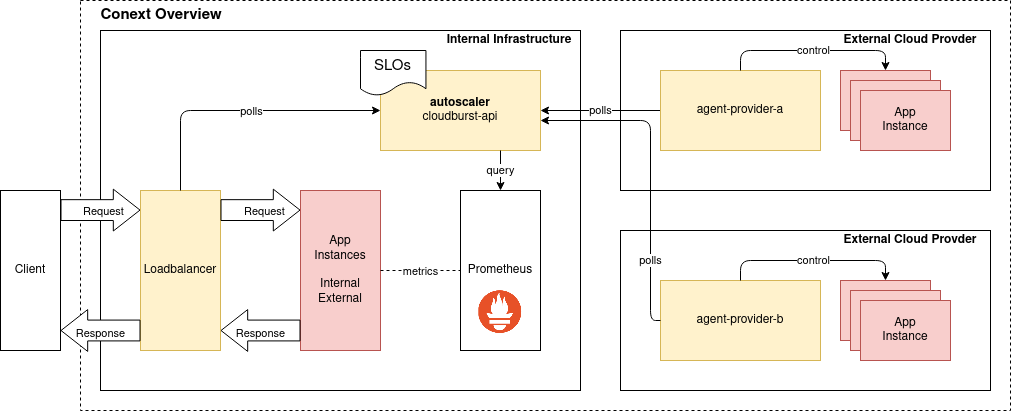
\includegraphics[width=1.0\linewidth,scale=1.0]{images/context.png}
	\caption{Systemarchitektur des entwickelten Autoscalers}
\end{figure}

\subsection{Datenmodell}
	
\subsection{Control Plane}
	
\begin{figure}[h]
	\centering
	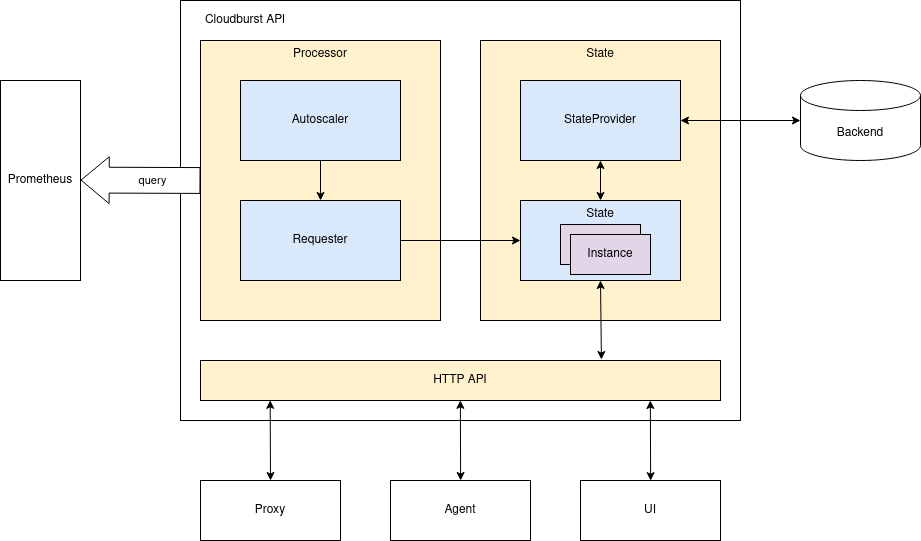
\includegraphics[width=1.0\linewidth,scale=1.0]{images/autoscaler.png}
	\caption{Hier muss was hin}
\end{figure}

\subsubsection{Configuration}
	
\subsubsection{Processor}
	
\subsubsection{Autoscaler}

\begin{figure}[h]
	\centering
	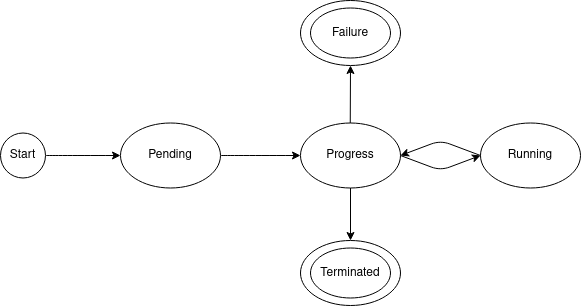
\includegraphics[width=0.8\linewidth,scale=0.8]{images/state.png}
	\caption{Hier muss was hin}
\end{figure}
	
\subsubsection{Requester}
	
\subsection{Agents}
	
\subsection{Proxy}

\subsection{Skalierungstechnik} \label{skalierungstechnik}

Requires expert knowledge about the dynamics of the ap-plication, including the service requirements of the appli-cation at each tier, and (ii) Requires sophisticated mod-eling expertise to determine when and how to resize thedeployment. For small and medium businesses (SMB),which comprise the targeted customer base for manycloud service providers (CSPs) [8,24], these hurdles arenon-trivial to overcome.

Many CSPs today offer monitoring services to users (notnecessarily for free) for tracking resource usage. Whilesuch monitoring services provide valuable information,the user still requires expert knowledge about the appli-cation and the performance modeling expertise to con-vert the monitored information into scaling actions.Some CSPs also offer rule-based triggers to help usersscale their applications. These rule-based triggers allowthe users to specify some conditions on the monitoredmetrics which, when met, will trigger a pre-defined scal-ing action.  Even with the help of rule-based triggers,however, the burden of determining the threshold condi-tions for the metrics still rests with the user. For example,in order to use a CPU utilization based trigger for scal-ing, the user must determine the CPU threshold at whichto trigger scale-up and scale-down, and the number ofinstances to scale-up and scale-down

% file:///home/chris/Zotero/storage/LUKLJ8WX/Gandhi%20et%20al.%20-%20Adaptive,%20Model-driven%20Autoscaling%20for%20Cloud%20Appli.pdf

\section{Experimente}
	
	
\section{Ausblick}
	
% ---- Bibliography ----
%
% BibTeX users should specify bibliography style 'splncs04'.
% References will then be sorted and formatted in the correct style.
%
\newpage
\bibliographystyle{splncs04}
\bibliography{paper.bib}
%
\end{document}
